\chapter{Methods and Materials}
\label{chp:MaM}

%%%%%%%%%%%%%%%%%%%%%%%%%%%%%%%%%%%%%%%%%%%%%%%%%%%%%%%%%%%%%%%%%%%%%%%
\section{Evolutionary Algorithm}
\label{sec:EA}

A population is run, evaluated and evolved for the number of generations specified.

Two parent population members are selected for evolution. Parents are ranked in descending order according to their fitness. The ranking procedure is discussed in detail in Section~\ref{sec:R}. The parent population is iterated through from the most fit to the least fit parent until a parent has been selected. A random number between 0 and 1 for selection is generated. A fitness weighting function is used to determine the selection of a parent. The fitness weighting function is defined as

\begin{equation}
	y=\frac{2\left ( p+1-r \right )^{c}}{p^{2}+p}
\end{equation}

Where

\begin{itemize}
	\item $y$ is the fitness weighting
	\item $p$ is the population size
	\item $r$ is the rank of the selected member
	\item $c$ is a user-defined fitness constant set to 1
\end{itemize}

The cumulative fitness weighting of all units before and after the current population member is calculated. If the random number is between the two cumulative fitness weightings, the member is selected as the parent.

Population members may evolve in three ways.

Crossover may occur between two parents. For every crossover point, a random number between 0 and 1 is generated. If the number is below the specified probability, crossover occurs. A random index in the list of parent parameters is selected. The parameters are swapped between parents from this index onwards. The two resulting children are potentially evolved further.

Random mutation of a child parameter may occur. For every random mutation point, a random number between 0 and 1 is generated. If the number is below the specified probability, random mutation occurs. A random parameter of the child is selected. The parameter is randomly changed to any allowed value for that parameter.

Biased mutation of a child parameter may occur. For every biased mutation point, a random number between 0 and 1 is generated. If the number is below the specified probability, biased mutation occurs. A random parameter of the child is selected. Another random number between 0 and 1 is generated. If the number is below 0.5, the parameter is decreased by 1. If the number is above or equal to 0.5, the parameter is increased by 1. The parameter is bounded by the allowed ranges.

All children are added to the population list. The new population list is used to generate the next population of units.

\section{L-Systems}
\label{sec:LS}

An L-System-like generation method is implemented due to the L-System features of efficiency, compactness and scalability. L-Systems are defined using class objects containing all necessary information.

\subsection{Parameters}

L-System class object parameters are

\begin{itemize}
	\item \textit{vocab} - The L-System vocabulary
	\item \textit{gramm} - The L-System grammar
	\item \textit{axiom} - The initial axiom of the L-System
	\item \textit{n} - The number of iterations to apply to the L-System
	\item \textit{seed} - The random generation seed used to generate the L-System if applicable
	\item \textit{word} - The resulting word of the L-System
\end{itemize}

The L-System vocabulary is itself a class object. The vocabulary is predefined. It consists of variables and constants. The vocabulary and its interpretations are outlined in Tables~\ref{tab:lsvarint} and~\ref{tab:lsconint}. The vocabulary is separated according to variables and constants. The vocabulary interpretation differs from traditional L-System interpretations. The interpretation is required to fill in elements of a grid. Traditional L-System interpretations result in lines of varying lengths and angles being drawn. A unique interpreter was designed and implemented for the purposes of this project.

% Please add the following required packages to your document preamble:
% \usepackage{booktabs}
\begin{table}[H]
\centering
\begin{tabular}{@{}cl@{}}
\toprule
\textbf{Variable} & \multicolumn{1}{c}{\textbf{Interpretation}}             \\ \midrule
F & \begin{tabular}[c]{@{}l@{}}Create an element at the current position and increment\\ the current position in the current direction\end{tabular} \\
f                 & Increment the current position in the current direction \\
+                 & Rotate the current direction by 45\textdegree  clockwise           \\
-                 & Rotate the current direction by 45\textdegree  counterclockwise    \\ \bottomrule
\end{tabular}
\caption{L-System variable interpretation}
\label{tab:lsvarint}
\end{table}

% Please add the following required packages to your document preamble:
% \usepackage{booktabs}
\begin{table}[H]
\centering
\begin{tabular}{@{}cl@{}}
\toprule
\textbf{Constant} & \multicolumn{1}{c}{\textbf{Interpretation}}                                                                                \\ \midrule
{[}               & Push the current position to the position memory stack                                                                     \\
{]}               & \begin{tabular}[c]{@{}l@{}}Pop the latest position on the position memory stack\\ and return to that position\end{tabular} \\
( &
  \begin{tabular}[c]{@{}l@{}}Push the current position to the position memory stack\\ All directional variables, i.e. + and -, in the word\\ following this constant are reversed until the )\\ constant is encountered\end{tabular} \\
)                 & \begin{tabular}[c]{@{}l@{}}Pop the latest position on the position memory stack\\ and return to that position\end{tabular} \\ \bottomrule
\end{tabular}
\caption{L-System constant interpretation}
\label{tab:lsconint}
\end{table}

Randomly generated L-Systems are manipulated using a random generation seed. Randomly generated L-Systems have requirements and specifications implemented to ensure the validity of the L-System.

At least one L-System rule must be defined. This rule must apply to the variable "F" and must itself contain at least one instance of the letter "F". Up to three additional rules may be defined, one for each of the remaining variables.

Rule components are selected from a predefined list included in Table~\ref{tab:lsrulecom}. Rule components were selected for various reasons. Rule components containing more than one character allow for variability in rule length. Rule components containing two identical directional variables specify 90\textdegree rotations. Rule components enclosed within square brackets allow for branches to exist within the L-System.

% Please add the following required packages to your document preamble:
% \usepackage{booktabs}
\begin{table}[H]
\centering
\begin{tabular}{@{}ccl@{}}
\toprule
\textbf{Number} &
  \textbf{\begin{tabular}[c]{@{}c@{}}Rule\\ Component\end{tabular}} &
  \multicolumn{1}{c}{\textbf{Interpretation}} \\ \midrule
1 &
  F &
  \begin{tabular}[c]{@{}l@{}}Create an element at the current position and\\ increment the current position in the current\\ direction\end{tabular} \\
2 &
  f &
  \begin{tabular}[c]{@{}l@{}}Increment the current position in the current\\ direction\end{tabular} \\
3 &
  + &
  Rotate the current direction by 45\textdegree  clockwise \\
4 &
  - &
  \begin{tabular}[c]{@{}l@{}}Rotate the current direction by 45\textdegree\\ counterclockwise\end{tabular} \\
5 &
  ++ &
  Rotate the current direction by 90\textdegree  clockwise \\
6 &
  -- &
  \begin{tabular}[c]{@{}l@{}}Rotate the current direction by 90\textdegree\\ counterclockwise\end{tabular} \\
7 &
  fF &
  2, then 1 \\
8 &
  Ff &
  1, then 2 \\
9 &
  {[}F{]} &
  \begin{tabular}[c]{@{}l@{}}Push the current position to the position\\ memory stack, then 1, then pop the latest\\ position on the position memory stack and\\ return to that position\end{tabular} \\
10 &
  {[}f{]} &
  \begin{tabular}[c]{@{}l@{}}Push the current position to the position\\ memory stack, then 2, then pop the latest\\ position on the position memory stack and\\ return to that position\end{tabular} \\
11 &
  {[}+F{]} &
  \begin{tabular}[c]{@{}l@{}}Push the current position to the position\\ memory stack, then 3, then 1, then pop the\\ latest position on the position memory stack\\ and return to that position\end{tabular} \\
12 &
  {[}+fF{]} &
  \begin{tabular}[c]{@{}l@{}}Push the current position to the position\\ memory stack, then 3, then 7, then pop the\\ latest position on the position memory stack\\ and return to that position\end{tabular} \\
13 &
  {[}-F{]} &
  \begin{tabular}[c]{@{}l@{}}Push the current position to the position\\ memory stack, then 4, then 1, then pop the\\ latest position on the position memory stack\\ and return to that position\end{tabular} \\
14 &
  {[}-fF{]} &
  \begin{tabular}[c]{@{}l@{}}Push the current position to the position\\ memory stack, then 4, then 7, then pop the\\ latest position on the position memory stack\\ and return to that position\end{tabular} \\ \bottomrule
\end{tabular}
\caption{L-System rule components and their interpretations}
\label{tab:lsrulecom}
\end{table}

During initial trials, many issues were encountered in allowing rules to be generated with single or unevenly matched brackets. The predefined L-System axioms contain square and round brackets. If rules contain single or unevenly matched brackets, the interpretation of the resulting word will not adhere to the specified symmetrical conditions.

Twelve axioms are predefined and outlined in Table~\ref{tab:lsaxiom}. Axioms were defined according to desirable symmetry conditions. Symmetry conditions are illustrated in Figures~\ref{fig:lssymex} and~\ref{fig:lssym}. 

% Please add the following required packages to your document preamble:
% \usepackage{booktabs}
\begin{table}[H]
\centering
\begin{tabular}{@{}lcc@{}}
\toprule
\multicolumn{1}{c}{\textbf{Axis}}                                        & \textbf{Rotational Axiom}           & \textbf{Reflective Axiom}   \\ \midrule
Horizontal        & {[}F{]}++++{[}F{]}   & {[}F{]}++++(F)   \\
Vertical          & -{}-{[}F{]}++++{[}F{]} & -{}-{[}F{]}++++(F) \\
\begin{tabular}[c]{@{}l@{}}Horizontal and\\ vertical\end{tabular}        & {[}F{]}++{[}F{]}++{[}F{]}++{[}F{]}  & {[}F{]}++(F)++{[}F{]}++(F)  \\
Diagonal          & +{[}F{]}++++{[}F{]}  & +{[}F{]}++++(F)  \\
Negative diagonal & -{[}F{]}++++{[}F{]}  & -{[}F{]}++++(F)  \\
\begin{tabular}[c]{@{}l@{}}Diagonal and\\ negative diagonal\end{tabular} & +{[}F{]}++{[}F{]}++{[}F{]}++{[}F{]} & +{[}F{]}++(F)++{[}F{]}++(F) \\ \bottomrule
\end{tabular}
\caption{L-System axioms}
\label{tab:lsaxiom}
\end{table}

\begin{figure}[H]
	\centering
	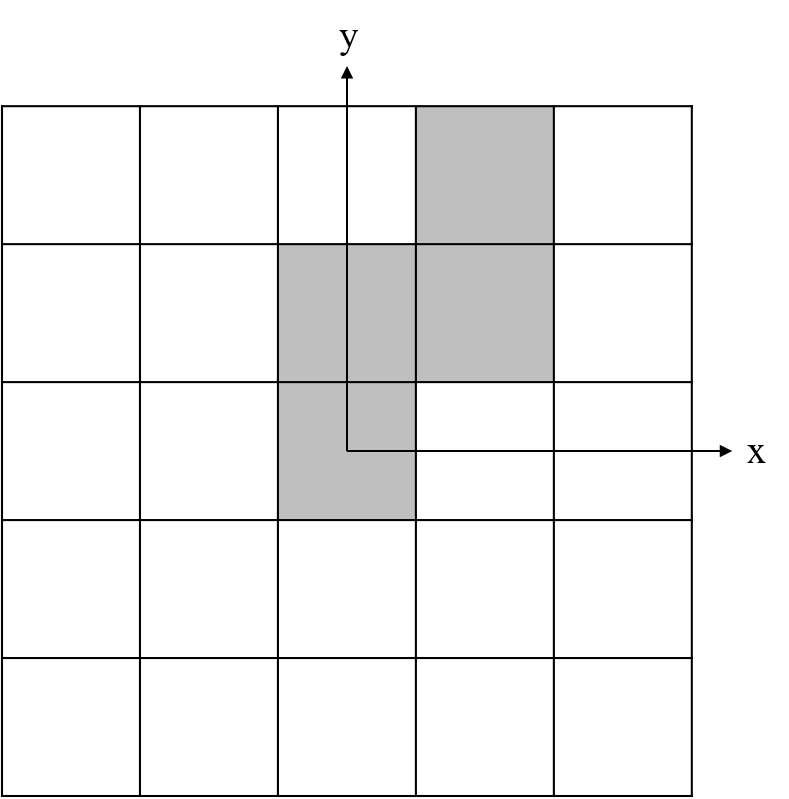
\includegraphics[width=0.5\textwidth]{LSSym.png}
	\caption{L-System symmetry interpretation example layout}
	\label{fig:lssymex}
\end{figure}

\begin{figure}[H]
	\centering
	\begin{subfigure}[t]{0.3\textwidth}
		\centering
		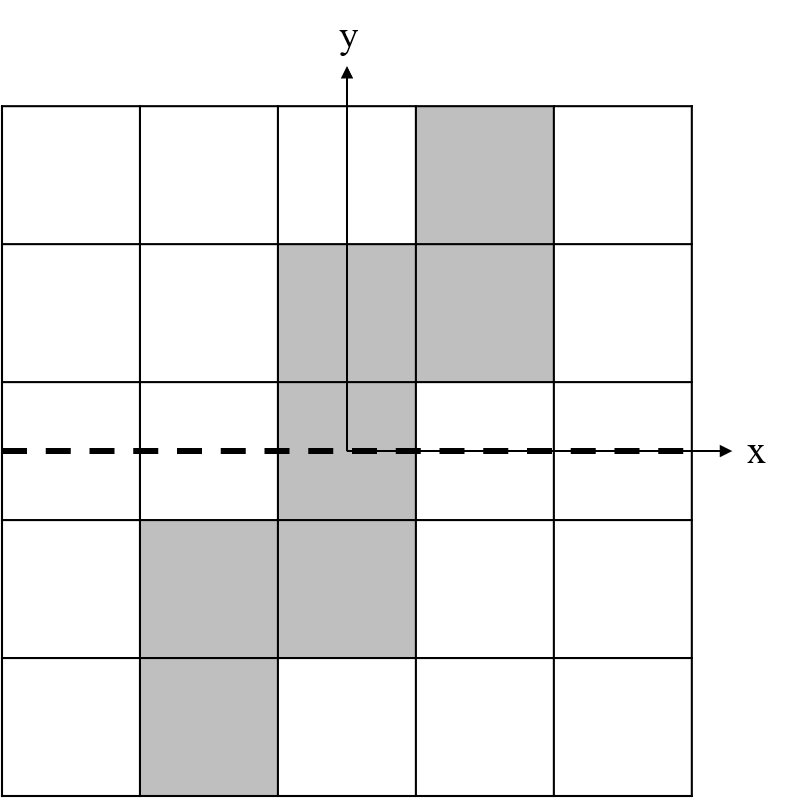
\includegraphics[width=\textwidth]{LSSymRotH.png}
		\caption{Horizontal rotation}
	\end{subfigure}
	\hfill
	\begin{subfigure}[t]{0.3\textwidth}
		\centering
		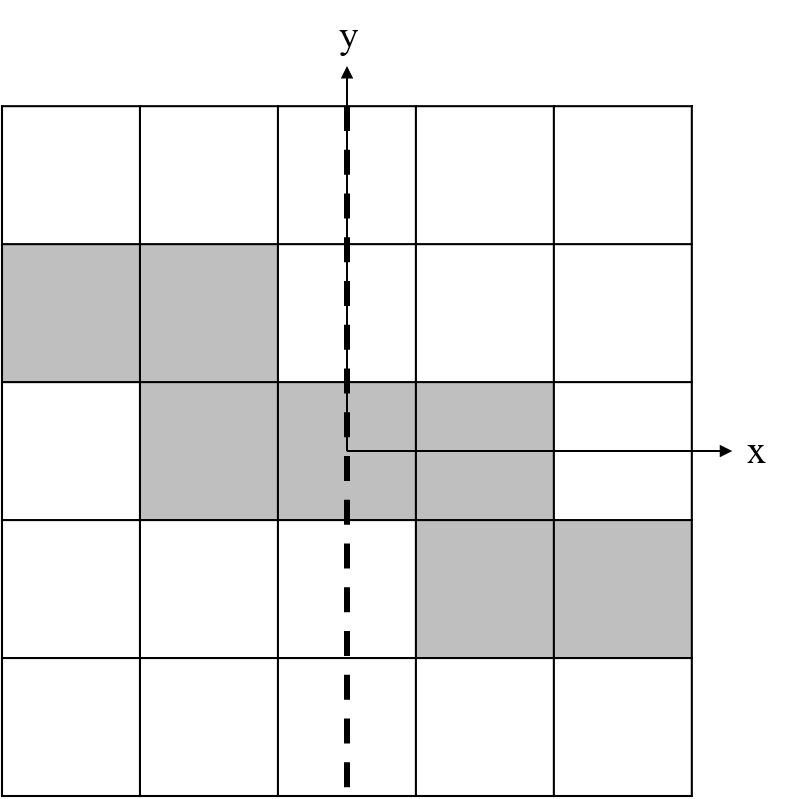
\includegraphics[width=\textwidth]{LSSymRotV.png}
		\caption{Vertical rotation}
	\end{subfigure}
	\hfill
	\begin{subfigure}[t]{0.3\textwidth}
		\centering
		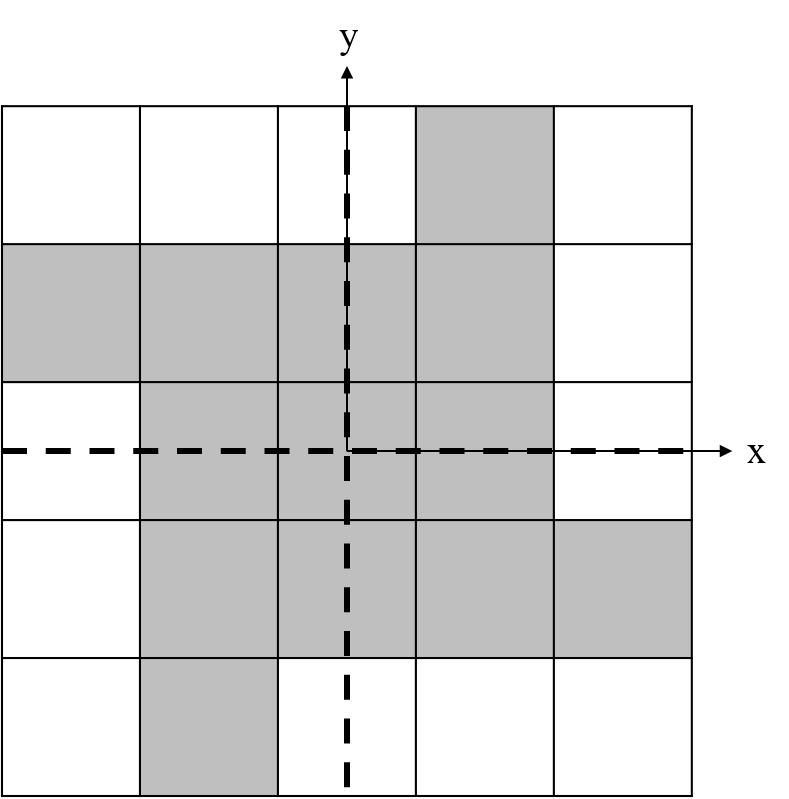
\includegraphics[width=\textwidth]{LSSymRotHV.png}
		\caption{Horizontal and vertical rotation}
	\end{subfigure}
	\hfill
	\begin{subfigure}[t]{0.3\textwidth}
		\centering
		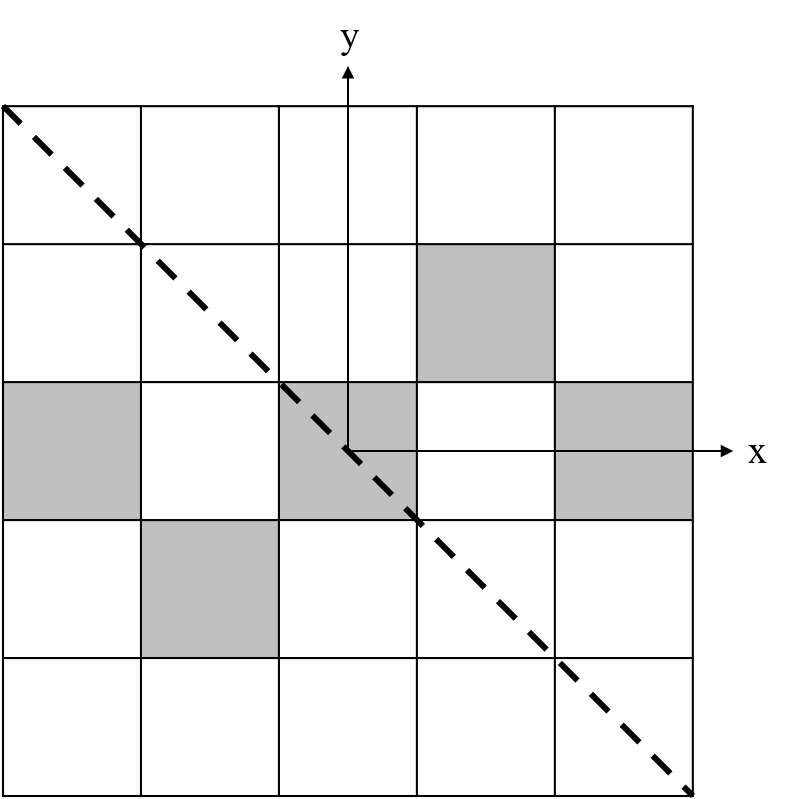
\includegraphics[width=\textwidth]{LSSymRotD.png}
		\caption{Diagonal rotation}
	\end{subfigure}
	\hfill
	\begin{subfigure}[t]{0.3\textwidth}
		\centering
		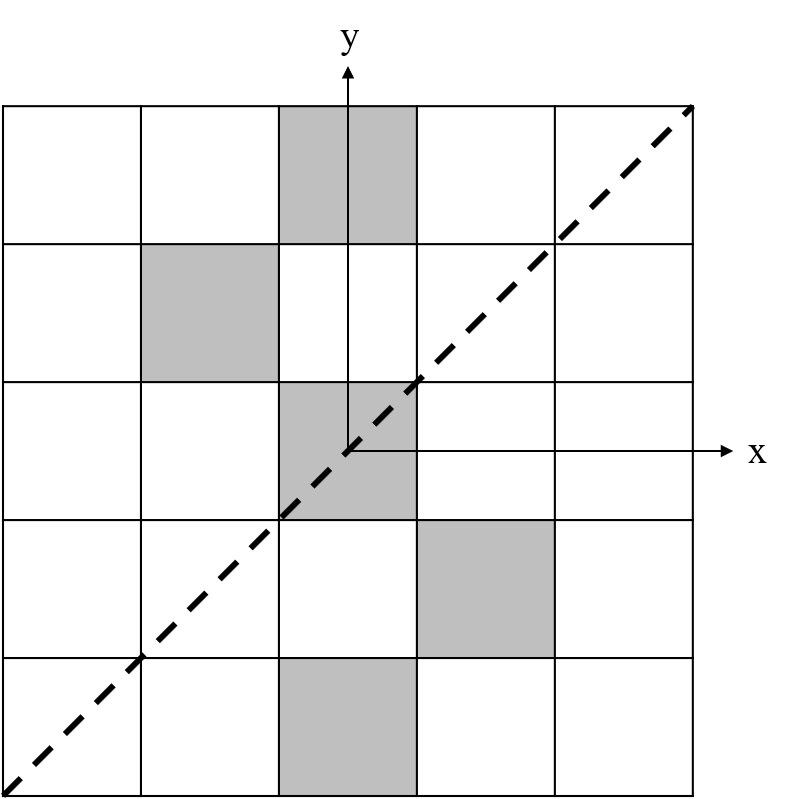
\includegraphics[width=\textwidth]{LSSymRotND.png}
		\caption{Negative diagonal rotation}
	\end{subfigure}
	\hfill
	\begin{subfigure}[t]{0.3\textwidth}
		\centering
		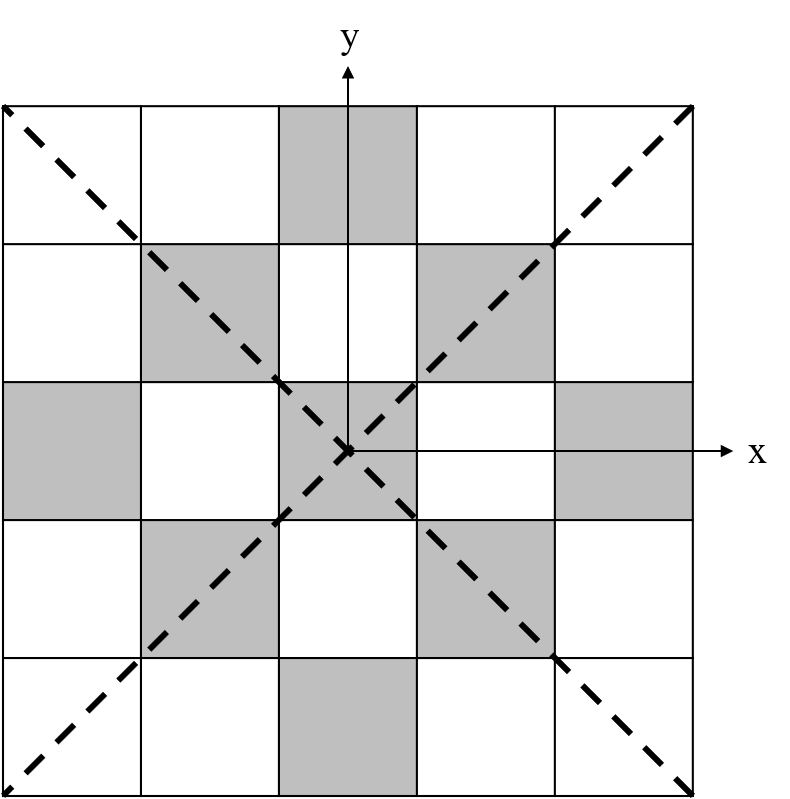
\includegraphics[width=\textwidth]{LSSymRotDND.png}
		\caption{Diagonal and negative diagonal rotation}
	\end{subfigure}
	\hfill
	\begin{subfigure}[t]{0.3\textwidth}
		\centering
		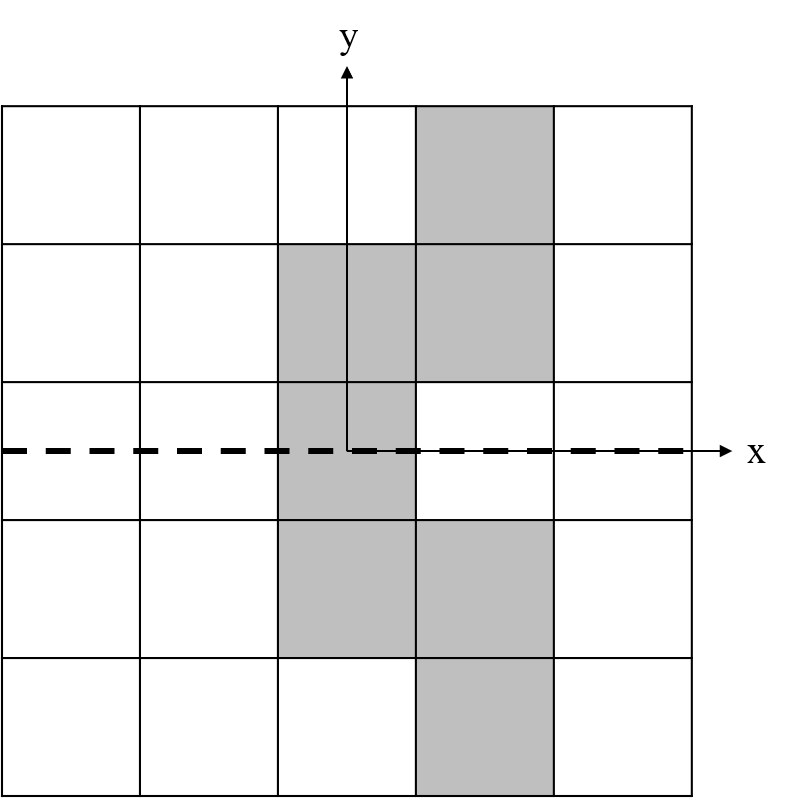
\includegraphics[width=\textwidth]{LSSymRefH.png}
		\caption{Horizontal reflection}
	\end{subfigure}
	\hfill
	\begin{subfigure}[t]{0.3\textwidth}
		\centering
		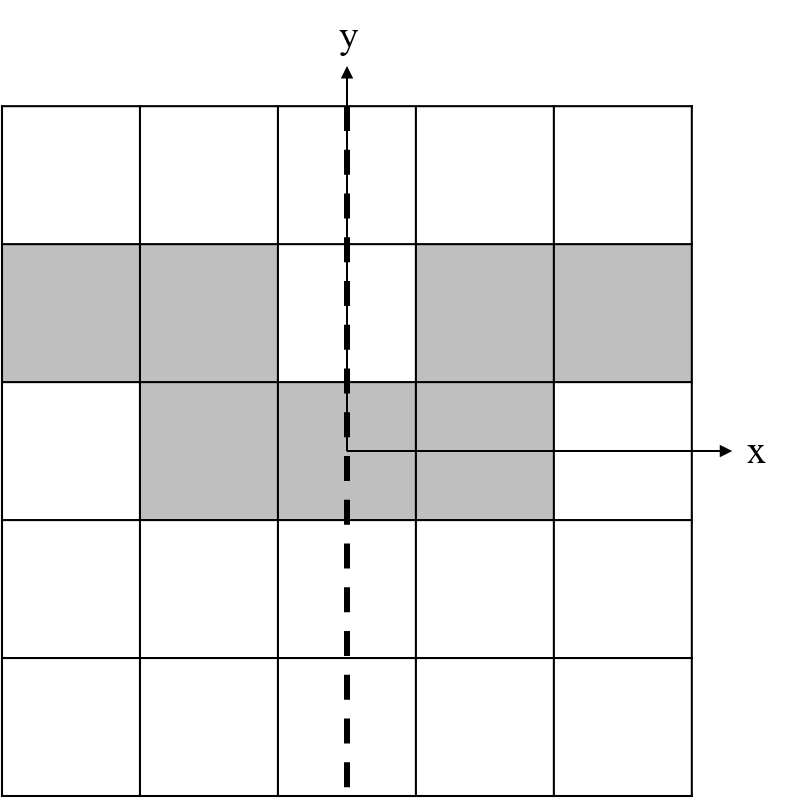
\includegraphics[width=\textwidth]{LSSymRefV.png}
		\caption{Vertical reflection}
	\end{subfigure}
	\hfill
	\begin{subfigure}[t]{0.3\textwidth}
		\centering
		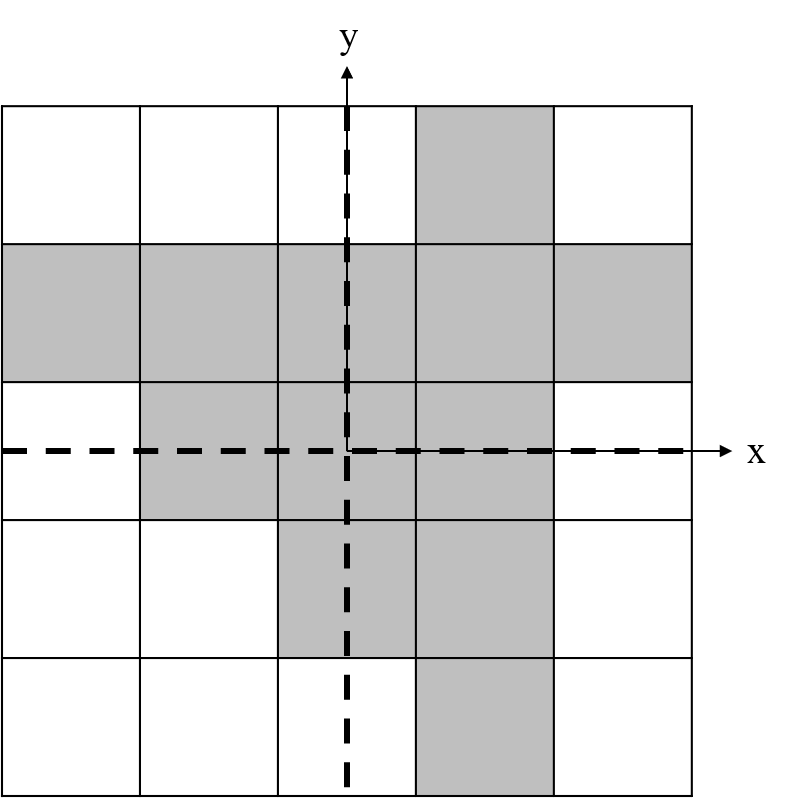
\includegraphics[width=\textwidth]{LSSymRefHV.png}
		\caption{Horizontal and vertical reflection}
	\end{subfigure}
	\hfill
	\begin{subfigure}[t]{0.3\textwidth}
		\centering
		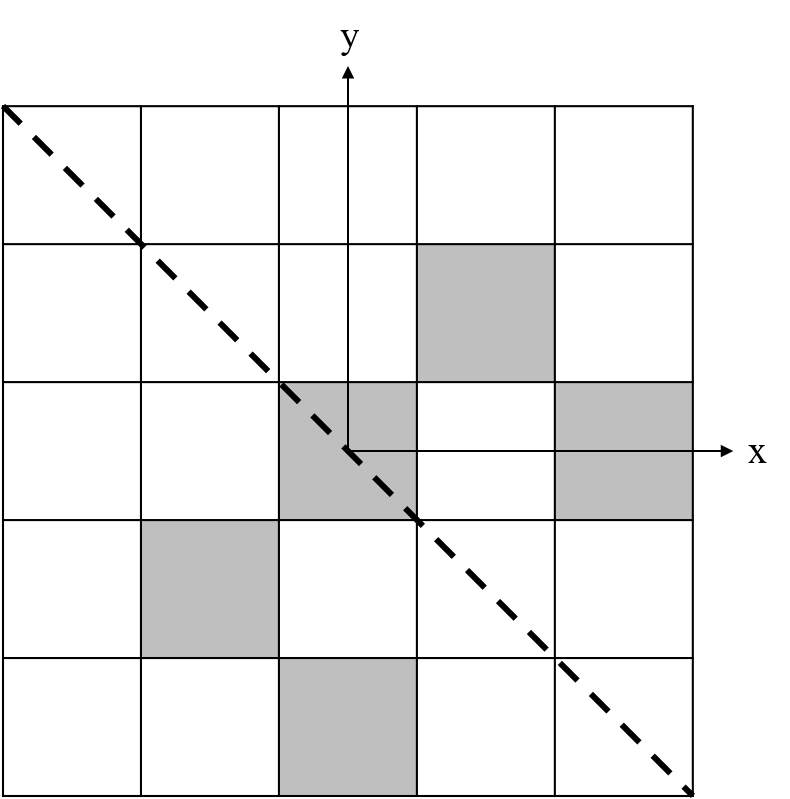
\includegraphics[width=\textwidth]{LSSymRefD.png}
		\caption{Diagonal reflection}
	\end{subfigure}
	\hfill
	\begin{subfigure}[t]{0.3\textwidth}
		\centering
		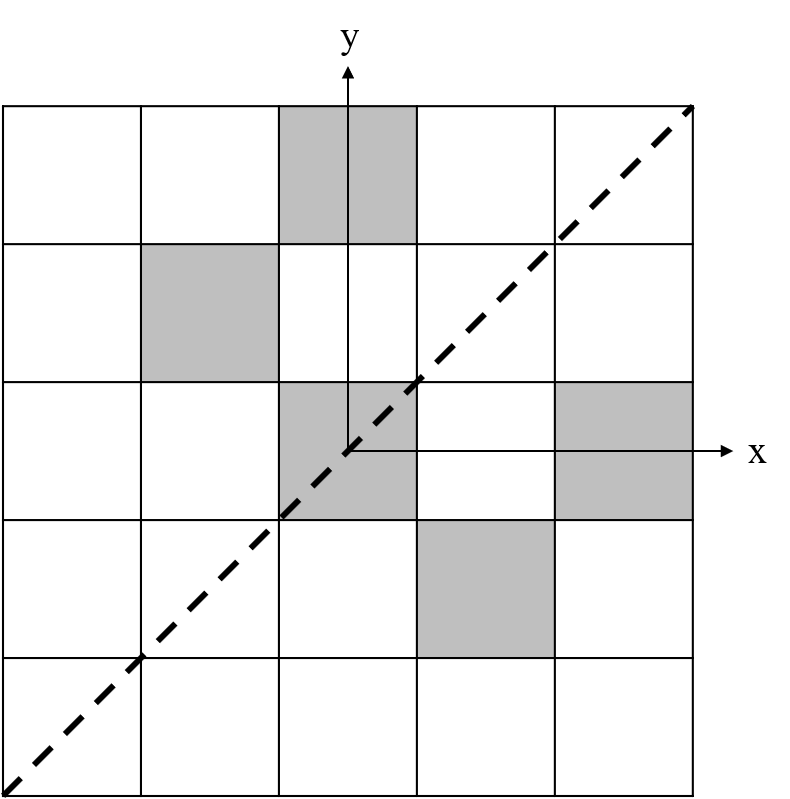
\includegraphics[width=\textwidth]{LSSymRefND.png}
		\caption{Negative diagonal reflection}
	\end{subfigure}
	\hfill
	\begin{subfigure}[t]{0.3\textwidth}
		\centering
		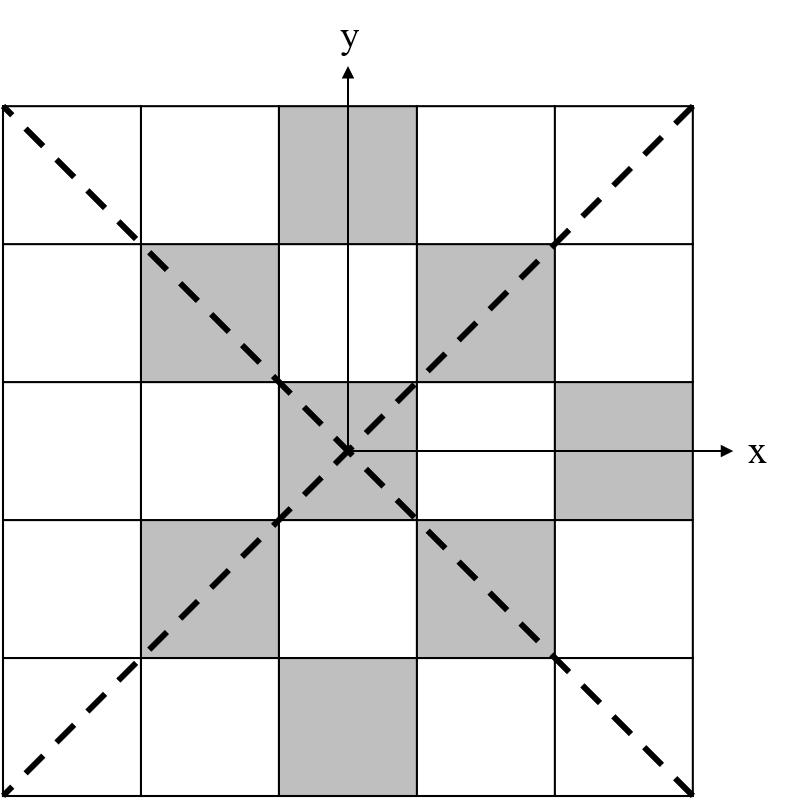
\includegraphics[width=\textwidth]{LSSymRefDND.png}
		\caption{Diagonal and negative diagonal reflection}
	\end{subfigure}
	\caption{L-System interpretation of symmetry axioms according to Figure~\ref{fig:lssymex}. Axes of symmetry are indicated with dotted lines}
	\label{fig:lssym}
\end{figure}

The true axiom is a single "F". All rules are applied for the specified number of iterations. The resulting word is placed within the axiom at all positions occupied by an "F". This allows for the symmetry conditions to be maintained across iterations while retaining "+" and "-" as variables.

\subsection{Interpretation}

The final word is interpreted according to the specified internal dimensions of the template. The word is interpreted character by character.

The number of open round brackets in the word is counted. For every open round bracket, the first subsequent closed round bracket is identified. Each string segment starting and ending with an open and closed round bracket is extracted. The round brackets are replaced with the equivalent square brackets. Pluses and minuses are swapped to invert all directional changes within the round brackets. This allows for reflection symmetry conditions to be applied. The original string segment is replaced with the adjusted string segment.

Every character in the word is interpreted from the initial character. The interpretation applies to a grid of squares identified by x- and y-coordinates. The origin square is defined by the coordinates (0, 0). Positive and negative directions are applied as per standard convention. The interpretation starts at the origin with the direction at 0\textdegree, i.e. in the positive y-direction.

\begin{figure}[H]
	\centering
	
\includegraphics[width=0.5\textwidth]{LSOrigin.png}
	\caption{Example 5x5 grid for L-System interpretation indicating the origin and orientation. The current position is outlined.}
	\label{fig:lso}
\end{figure}

If the character is "F", a check is done to determine if the stack is at its initial value or if the current element is the initial element. If it is either, the element coordinates are set to the origin. If it is neither, the x- and y-coordinates are incremented in the current direction. The new element coordinates are added to the list of coordinates.

If the character is "f", the procedure is identical to the procedure for the character "F", except that the new element coordinates are not added to the list of coordinates. Thus the position is incremented without an element being added.

\begin{figure}[H]
	\centering
	\begin{subfigure}[c]{0.4\textwidth}
		\centering
		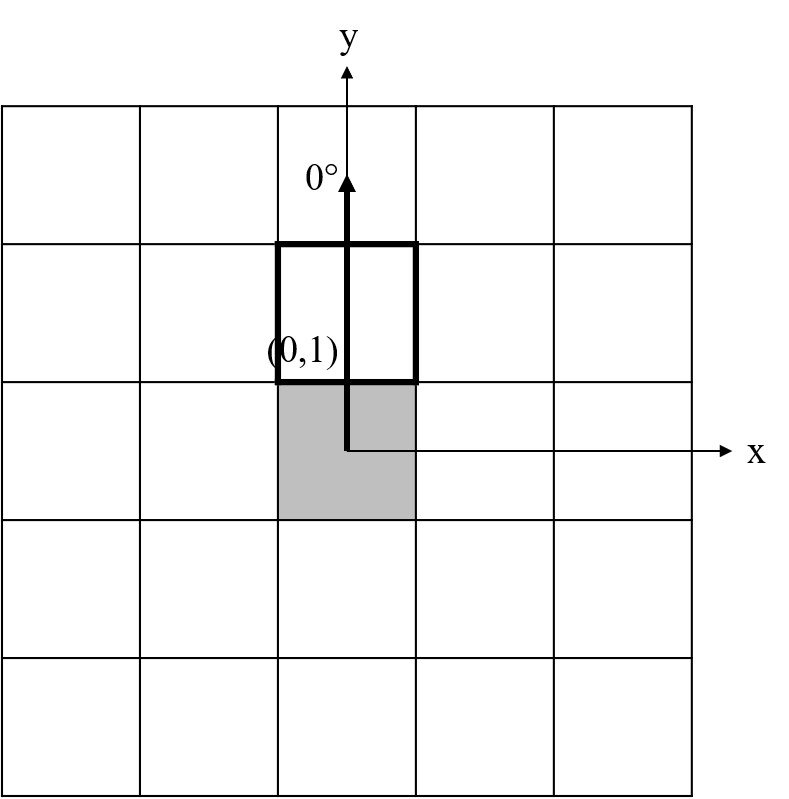
\includegraphics[width=\textwidth]{LSF.png}
		\caption{Interpretation of "F" from the origin. A saved element is filled in.}
	\end{subfigure}
	\hfill
	\begin{subfigure}[c]{0.4\textwidth}
		\centering
		
\includegraphics[width=\textwidth]{LSfsmall.png}
		\caption{Interpretation of "f" from the origin.}
	\end{subfigure}
	\caption{L-System interpretation of movement variables}
	\label{fig:lsmove}
\end{figure}

If the character is "+", the current direction is incremented by 45\textdegree. If the character is "-", the current direction is decremented by 45\textdegree.

\begin{figure}[H]
	\centering
	\begin{subfigure}[c]{0.4\textwidth}
		\centering
		
\includegraphics[width=\textwidth]{LS+.png}
		\caption{Interpretation of "+" from the origin}
	\end{subfigure}
	\hfill
	\begin{subfigure}[c]{0.4\textwidth}
		\centering
		
\includegraphics[width=\textwidth]{LS-.png}
		\caption{Interpretation of "-" from the origin}
	\end{subfigure}
	\caption{L-System interpretation of rotational variables}
	\label{fig:lsrot}
\end{figure}

If the character is "[", the current position and direction is added to the stack. If the character is "]", a check is done to determine if the stack is at its initial value. If it is, the initial coordinates and direction are fetched. If it is not, the latest coordinates and direction are popped from the stack. A check is then done to determine if the stack is at its initial position. If it is, a flag is set to indicate as such.

The complete list of coordinates is sorted in ascending order. All duplicate element coordinates are removed. The coordinates are shifted from centering around the origin to centering around the central element of the unit. All coordinates outside of the internal space of the unit are dropped. The remaining coordinates are interpreted as element indices. The element indices are compared to the list of all internal element indices and the list of elements to be removed is obtained.

\section{CPPNs}
\label{sec:CPPN}

An CPPN-like generation method is implemented due to the CPPN features of image generation and scalability. CPPNs are defined using class objects containing all necessary information. CPPN class object parameters are:

\begin{itemize}
	\item \textit{seed} - The random generation seed used to generate the CPPN
	\item \textit{mod\_n} - The number of models to be generated by the CPPN
	\item \textit{scale} - The scale of the focus on the model
	\item \textit{hl\_n} - The number of hidden layers in the network
	\item \textit{hl\_s} - The size of the initial hidden layer
	\item \textit{thresh} - The rounding or element removal threshold
	\item \textit{x} - The number of elements in the x-direction
	\item \textit{y} - The number of elements in the y-direction
\end{itemize}

A random generation seed is used to determine the CPPN's initial layer, hidden layers, and activation functions. The random generation seed allows for replicability of CPPNs.

A single CPPN may generate a number of models. A CPPN model is defined as a class object containing the relevant information. CPPN model class object parameters are

\begin{itemize}
	\item \textit{cppn} - The CPPN class object used to generate the model
	\item \textit{mod\_id} - The model ID
	\item \textit{grid} - The binary model grid
\end{itemize}

A CPPN model may be scaled inwards or outwards. The scale parameter was set at 1, i.e. no scaling, in order to reduce complexity. The functionality of the scaling was left implemented to allow for future tests.

The threshold parameter allows for two approaches to the removal of elements. The CPPN outputs 2D arrays of values ranging from 0 to 1. If the threshold parameter is set from 0 to 1, it is interpreted as a rounding threshold. All values above or equal to the threshold are set to 1 and all values below or equal to the threshold are set to 0. If the threshold parameter is set above 1 to 100, it is interpreted as a percentage of elements to remove. The lowest values making up the specified percentage of all values are set to 0 and the rest of the values are set to 1.

The x- and y-dimensions are specified initially. All hidden layers barring the initial layer have a number of nodes equal to the x-dimension multiplied with the y-dimension. The CPPN will result in a model that fits perfectly within the internal space of the unit.

CPPN models obtained for the purposes of this this thesis are at much lower resolutions than traditional CPPN models. A reduction in complexity was deemed appropriate. Traditional CPPNs allow for unique activation functions to be applied to each node. This was not implemented in order to reduce complexity. Five activation functions are available for the hidden layers of the CPPN. Activation functions are applied to an entire layer. The activation functions are

\begin{itemize}
	\item sin
	\item cos
	\item tanh
	\item sigmoid
	\item smooth ReLu
\end{itemize}

Only the last two activation functions are available for the output layer of the CPPN. They result in values ranging only from 0 to 1.

\section{Software}
\label{sec:SW}

The software pipeline is complex, and many components are interrelated. Details considered trivial or irrelevant are not discussed. The entirety of the code is available to the reader if they would wish to investigate or make use of it. The code is extensively commented for any clarification needed.

\subsection{Software Selection}

The Finite Element Method (FEM) is an approach to numerically solving field problems. Field problems require the determination of one or more dependent variables' distribution in space. Field problems are mathematically described with differential equations or integral expressions. Finite elements can be expressed as small parts of a larger body. A field quantity within an element may only have a simple spatial variation, such as being described by polynomial terms no higher than the second order. FEM differs from calculus as calculus uses infinitesimal elements. FEM thus delivers approximate solutions. \cite{Cook2002}

Several commercial FEM software packages capable of realistically modeling soft bodies are available. LSDyna is a FEM software package widely used in industry. It is owned by ANSYS and maintained by LSTC. The software's code is based on highly non-linear and transient dynamic FEM with explicit time integration \cite{LSDyna}. Siemens NX 12 is an integrated software package capable of performing FEM analysis. The software package has a user-friendly interface for graphical design of components \cite{NX12}. MSC.Marc Mentat is a pre- and postprocessing software for the MSC.Marc FEM solver. It is focused on nonlinear material modeling and analysis. It has an extensive set of options available for post-processing \cite{MSC}. MSC.Marc Mentat 2019 is selected for this project.

Python 3.6 is used to construct a modelling pipeline. Packages are available that allow for the integration of Python and Marc. Many advanced numerical analysis packages are also available for Python.

\subsection{Template}

The generative design approach as implemented requires large populations of similar units to be created and run. The units need to be similar to meaningfully draw comparisons between them and select the best performing units. A template unit is created containing all necessary and non-unique specifications. The template has all appropriate FEM settings applied. The template can be altered according to the specified design methodology.

The template is a 2D grid of square elements. 2D quad shell elements are used. The template has boundary conditions applied causing deformation according to a specified case. Cases are outlined in Section.

Template parameters need to be specified by the user. Relevant template parameters include:

\begin{itemize}
	\item \textit{case} - The template case identifier
	\item \textit{x\_e} - The number of elements in the x-direction 
	\item \textit{y\_e} - The number of elements in the y-direction
	\item \textit{e\_s} - The side length of the element in mm
	\item \textit{b} - The number of elements reserved for the unit boundary width
	\item \textit{ogd\_mat} - The Ogden material model parameters
	\item \textit{n\_steps} - The number of analysis steps in the second of analysis
	\item \textit{table\_name} - The name of the function applied to the template
	\item \textit{d\_mag} - The applied displacement in mm
	\item \textit{p\_mag} - The applied internal pressure in MPa
\end{itemize}

The template case identifier refers to one of three deformation cases applied to the template. These cases are discussed in detail in Section~\ref{sec:UC}.

The user-specified template parameters are used to define a template class object. The template class object calculates more parameters used in the construction of the template. The relevant calculated parameters are outlined in Table~\ref{tab:tempcalcpar}.

% Please add the following required packages to your document preamble:
% \usepackage{booktabs}
\begin{table}[H]
\centering
\begin{tabular}{@{}lcl@{}}
\toprule
\textbf{Variable}    & \multicolumn{1}{l}{\textbf{Formula}} & \textbf{Description}                                                                                      \\ \midrule
\textit{x\_s}        & $e\_s\times x\_e$                    & \begin{tabular}[c]{@{}l@{}}The side length of the template\\ in mm in the x-direction\end{tabular}        \\
\textit{y\_s}        & $e\_s\times y\_e$                    & \begin{tabular}[c]{@{}l@{}}The side length of the template\\ in mm in the y-direction\end{tabular}        \\
\textit{ogd\_mat}    &                                      & \begin{tabular}[c]{@{}l@{}}The non-linear Ogden material\\ model\end{tabular}                             \\
\textit{x\_n}        & $x\_e+1$                             & \begin{tabular}[c]{@{}l@{}}The number of nodes in the\\ x-direction\end{tabular}                          \\
\textit{y\_n}        & $y\_e+1$                             & \begin{tabular}[c]{@{}l@{}}The number of nodes in the\\ y-direction\end{tabular}                          \\
\textit{n\_e}        & $x\_e\times y\_e$                    & \begin{tabular}[c]{@{}l@{}}The total number of elements\\ in the template\end{tabular}                    \\
\textit{n\_n}        & $x\_n\times y\_n$                    & \begin{tabular}[c]{@{}l@{}}The total number of nodes in the\\ template\end{tabular}                       \\
\textit{e\_internal} &                                      & \begin{tabular}[c]{@{}l@{}}The list of internal element IDs\\ that are allowed to be removed\end{tabular} \\
\textit{n\_external} &                                      & The list of external node IDs                                                                             \\
\textit{t\_id} &
  \begin{tabular}[c]{@{}c@{}}\textless{}\textit{case}\textgreater{}\_\textless{}\textit{x\_e}\textgreater{}x\textless{}\textit{y\_e}\textgreater\\ \_\textless{}\textit{x\_s}\textgreater{}x\textless{}\textit{y\_s}\textgreater{}\end{tabular} &
  The template ID \\
\textit{grid}        &                                      & A representative grid of ones                                                                             \\ \bottomrule
\end{tabular}
\caption{Calculated and internal template class object parameters}
\label{tab:tempcalcpar}
\end{table}

The template is then created in MarcMentat. The nodes are created starting at the global origin on the XY-plane. The nodes are incrementally added in the positive x-direction. The nodes are spaced apart as defined by \textit{e\_s}. Once a row of nodes is completed as defined by \textit{x\_n}, the y-coordinate is positively incremented as defined by \textit{e\_s}. A new row of nodes is created. This process is repeated until completed as defined by \textit{y\_n}.

Four nodes are used to make square 2D elements. Starting at the global origin, elements are incrementally added in the x-direction until completed as defined by \textit{x\_e}. All rows are added until completed as defined by \textit{y\_e}.

The graph used to apply the boundary conditions is defined. The boundary conditions are applied according to the case identifier. The boundary conditions related to each case are detailed in Section~\ref{sec:UC}.

Mechanical planar strain geometric properties are added to all elements. The Ogden material model for Mold-Star 15 is applied to all elements. A single contact body is defined containing all elements. The loadcase containing the fixed and forced displacement boundary conditions is created. The job for the loadcase is created.

The template is saved at this point. All units created during a simulation are built from this template. The template job is run and its success evaluated. The process of running a simulation and evaluating its success is outlined in Section~\ref{ssec:run}.

The template model is saved again. Meaningful template parameters and data obtained from the template is written in a human-readable manner to a log file. The template class object is saved to a file that can be accessed later.

\subsection{Analysis Approach}

The analysis approach is user-specified. Two analysis methods are available: a Monte Carlo-styled analysis and an evolutionary algorithm-based analysis. For the Monte Carlo-styled analysis, the user must specify the unit generation method and the number of units to be generated. For the evolutionary algorithm, the user-specified parameters are:

\begin{itemize}
	\item \textit{gen} - The number of generations
	\item \textit{prob} - The probabilities of an occurrence of crossover, random mutation, and biased mutation
	\item \textit{point} - The potential number of occurrences per unit of crossover, random mutation, and biased mutation
	\item \textit{meth} - The unit generation method
\end{itemize}

A population of units is generated according to the specified unit generation method. The unit generation process is outlined in Section~\ref{ssec:ug}. Both analysis methods use the same approach to the initial population generation.

A list of maximum and minimum parameter values is defined. The parameter values are appropriate to the unit generation method specified. The different parameters, ranges and motivations are outlined in Table~\ref{tab:ungenmethpar}. The range values are inclusive.

% Please add the following required packages to your document preamble:
% \usepackage{booktabs}
% \usepackage{multirow}
% \usepackage{graphicx}
\begin{table}[H]
\centering
\resizebox{\textwidth}{!}{%
\begin{tabular}{@{}lccl@{}}
\toprule
\multicolumn{1}{c}{\multirow{2}{*}{\textbf{Parameter}}} &
  \multicolumn{2}{c}{\textbf{Range}} &
  \multicolumn{1}{c}{\multirow{2}{*}{\textbf{Motivation}}} \\ \cmidrule(lr){2-3}
\multicolumn{1}{c}{} &
  \textbf{Min} &
  \textbf{Max} &
  \multicolumn{1}{c}{} \\ \midrule
\multicolumn{4}{c}{\textbf{Random}} \\ \midrule
Seed &
  1 &
  \begin{tabular}[c]{@{}c@{}}Number of units\\ to be generated\end{tabular} &
  \begin{tabular}[c]{@{}l@{}}The seed is limited to the number of\\ units requested by the simulation\end{tabular} \\
\begin{tabular}[c]{@{}l@{}}Number of \\ elements removed\end{tabular} &
  0 &
  \begin{tabular}[c]{@{}c@{}}Number of\\ internal elements\end{tabular} &
  \begin{tabular}[c]{@{}l@{}}The complete range of elements which\\ may potentially be removed is included\end{tabular} \\ \midrule
\multicolumn{4}{c}{\textbf{L-System}} \\ \midrule
Seed &
  1 &
  \begin{tabular}[c]{@{}c@{}}Number of units\\ to be generated\end{tabular} &
  \begin{tabular}[c]{@{}l@{}}The seed is limited to the number of\\ units requested by the simulation\end{tabular} \\
Axiom ID &
  1 &
  \begin{tabular}[c]{@{}c@{}}Number of\\ predefined axioms\end{tabular} &
  The complete list of axioms is included \\
Number of rules &
  1 &
  \begin{tabular}[c]{@{}c@{}}Number of\\ L-System variables\end{tabular} &
  \begin{tabular}[c]{@{}l@{}}At least one rule is required for a valid\\ L-System, and the number of rules is\\ limited to the number of L-System variables\end{tabular} \\
Rule length &
  2 &
  5 &
  \begin{tabular}[c]{@{}l@{}}A rule must be longer than one character,\\ and potential complexity is limited\end{tabular} \\
\begin{tabular}[c]{@{}l@{}}Number of\\ iterations\end{tabular} &
  1 &
  5 &
  \begin{tabular}[c]{@{}l@{}}At least one iteration must be applied for a\\ valid L-System, and potential complexity is\\ limited\end{tabular} \\ \midrule
\multicolumn{4}{c}{\textbf{CPPN}} \\ \midrule
Seed &
  1 &
  \begin{tabular}[c]{@{}c@{}}Number of units\\ to be generated\end{tabular} &
  \begin{tabular}[c]{@{}l@{}}The seed is limited to the number of units\\ requested by the simulation\end{tabular} \\
Model ID &
  1 &
  N/A &
  Potential complexity is limited \\
Scale &
  1 &
  N/A &
  Potential complexity is limited \\
\begin{tabular}[c]{@{}l@{}}Number of\\ hidden layers\end{tabular} &
  2 &
  10 &
  \begin{tabular}[c]{@{}l@{}}At least two layers are required to have a\\ valid network, and potential complexity is\\ limited\end{tabular} \\
\begin{tabular}[c]{@{}l@{}}Size of the initial\\ hidden layer\end{tabular} &
  2 &
  32 &
   \\
\begin{tabular}[c]{@{}l@{}}Element removal\\ threshold\end{tabular} &
  0 &
  100 &
  \begin{tabular}[c]{@{}l@{}}The complete range of elements which\\ may potentially be removed is included\end{tabular} \\ \bottomrule
\end{tabular}%
}
\caption{Unit generation method parameter ranges and motivations}
\label{tab:ungenmethpar}
\end{table}

A population is randomly generated. Each population member is a list of parameters within the bounds specified in Table above. If the unit generation method is random, the two parameters are used to generate a list of elements to be removed directly. If the unit generation method is specified as L-Systems, the parameters are used to generate a random L-System. The L-System word is interpreted to obtain a list of elements to be removed. If the unit generation method is specified as CPPNs, the parameters are used to generate a random CPPN. The CPPN is set to generate the maximum number of models specified by the parameter. A CPPN model class object is defined with the model ID specified by the current parameters. The CPPN model class object is interpreted to obtain a list of elements to be removed.

Each list of elements to be removed is paired with the relevant class object or set of parameters. Each pair is added to the population list. The population list is used to create the units in Marc Mentat and run them.

The units are ranked according to performance metrics specified by the template case. A ranked list of the unit IDs is provided in descending order in a text file. The ranking process is discussed in more detail in Section~\ref{ssec:rank}. If the analysis approach was specified as Monte Carlo, the analysis stops here. Further evaluation of unit performance may be carried out by manual inspection.

If the analysis approach was specified as evolutionary algorithms, the process continues according to the evolutionary algorithm outlined in Section~\ref{sec:EA}.

\subsection{Unit Generation}
\label{ssec:ug}

Unit generation refers to the process of automatically specifying internal geometry of a unit based on the predefined template. Three methods of unit generation are implemented and investigated. All three methods provide a list of internal element IDs provided to MarcMentat as elements to be removed from the template file.

Random generation is implemented as a baseline to compare with the other two unit generation methods. A random generation seed is used to allow for replicability. A number of elements to be removed is first selected. This number has a possible range of zero to all internal elements. A list of unique internal element IDs is then selected and sorted.

L-Systems and CPPNs as outlined in Sections~\ref{sec:LS} and~\ref{sec:CPPN} respectively are also available for unit generation.

\subsection{Running a Job}
\label{ssec:run}

The command to run the job is sent to Marc Mentat. Jobs may take anywhere from 0.01 seconds to 300 seconds to complete. This depends on the complexity of the model and the number of cut-backs during calculation required to accurately solve for the model behavior.

Marc Mentat creates several files during the process of running a job. The log file specifies the exit condition of the job. The log file is not created at the start of the job.

A model is always saved just before a job is run. The time stamp of this saved model is used for evaluation of the log file. It is first determined if the log file exists. If it does not exist, the code waits for 1 second before checking again. This repeats until the log file is found to exist. If the log file is found, its time stamp is compared to the model file's time stamp. If the log file is older than the model, i.e. it is a log file of a previous run of the model, the code waits 1 second before checking if it has been updated. If the log file is newer than the model, it is inspected for the exit number string or the access violation string.

If the exit number string is found, the exit number is evaluated. Two exit numbers and an error case are identified and defined in Table~\ref{tab:exno}.

% Please add the following required packages to your document preamble:
% \usepackage{booktabs}
% \usepackage[normalem]{ulem}
% \useunder{\uline}{\ul}{}
\begin{table}[H]
\centering
\begin{tabular}{@{}cl@{}}
\toprule
\textbf{Exit Number} & \multicolumn{1}{c}{\textbf{Description}}       \\ \midrule
3004                 & A successful run                               \\
67                   & A license server connection timeout or failure \\
Other                & An unsuccessful run                            \\ \bottomrule
\end{tabular}
\caption{Marc Mentat exit number descriptions}
\label{tab:exno}
\end{table}

If exit number 3004 is found, the model is recognized as having run successfully. The model output file is opened. All relevant data is read from the model output file and written to clearly labeled CSV files. Any relevant data that must be calculated externally from Marc Mentat is calculated and also written to clearly labeled CSV files. Relevant data is outlined and motivated in Section .

If exit number 67 is found, the job is rerun and the entire process as detailed above is repeated until the exit number can be rerun again. If an access violation string is found, it is treated identically to exit number 67.

If any other exit number is found, an error message with the number is displayed. No results are obtained from the model. The model ID is logged appropriately.

The model is saved and the template model is reopened. The code continues on to the next model.

\subsection{Ranking}
\label{ssec:rank}

Unit performance measures are weighted equally. In order to compare them equivalently, all performance measures are normalized according to

\begin{equation}
	f=\frac{x-mean}{std}
\end{equation}

Where

\begin{itemize}
	\item $f$ is the fitness value
	\item $x$ is the performance measure
	\item $mean$ is the mean of all units' performance measures
	\item $std$ is the standard deviation of all units' performance measures
\end{itemize}

All fitness values applicable to a unit are summed together. Units are ranked in descending order according to the fitness value. The unit with the largest fitness value is deemed the most fit.

\section{Unit Deformation Cases}
\label{sec:UC}

\subsection{Uniaxial Elongation}

Case 1 is a case of uniaxial elongation as defined by Kim \cite{Kim2015}. This case has no rigid body modes. This case has applications in causing extension. Four boundary conditions are applied. They are outlined in Table~\ref{tab:c1}.

% Please add the following required packages to your document preamble:
% \usepackage{booktabs}
\begin{table}[H]
\centering
\begin{tabular}{@{}lllc@{}}
\toprule
\multicolumn{1}{c}{\textbf{Label}} & \multicolumn{1}{c}{\textbf{Boundary}} & \multicolumn{1}{c}{\textbf{Constraint}} & \textbf{Direction} \\ \midrule
\textit{bc\_fd\_yy1} & Bottom edge & Fixed               & y \\
\textit{bc\_fd\_yy2} & Top edge    & Forced displacement & y \\
\textit{bc\_fd\_xx1} & Left edge   & Fixed               & x \\
\textit{bc\_fd\_xx2} & Right edge  & Fixed               & x \\ \bottomrule
\end{tabular}
\caption{Uniaxial elongation boundary conditions \cite{Kim2015}}
\label{tab:c1}
\end{table}

The boundary conditions as applied in Marc Mentat to a template of 5x5 elements are illustrated in Figure~\ref{fig:c1bc}. The resulting deformation is illustrated in Figure~\ref{fig:c1def}. The original shape is outlined in pink.

\begin{figure}[H]
	\centering
	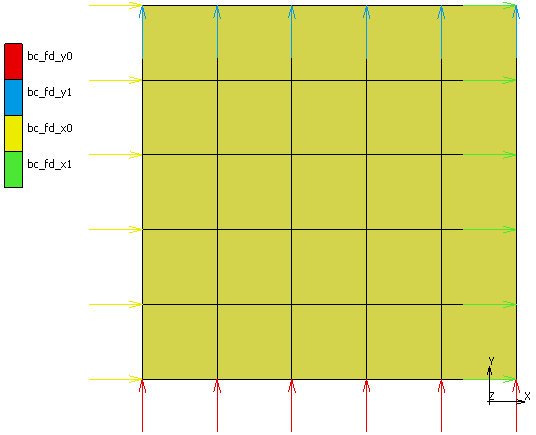
\includegraphics[width=0.5\textwidth]{C1BC.png}
	\caption{Uniaxial elongation boundary conditions as applied in Marc Mentat}
	\label{fig:c1bc}
\end{figure}

\begin{figure}[H]
	\centering
	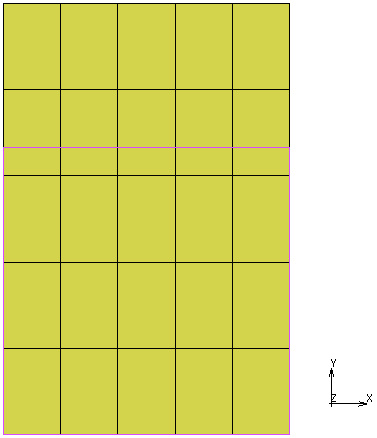
\includegraphics[width=0.5\textwidth]{C1Def.png}
	\caption{Resulting deformation of uniaxial elongation}
	\label{fig:c1def}
\end{figure}

\subsection{Biaxial Elongation}

Case 2 is a case of biaxial elongation. This case has applications in causing expansion. Four boundary conditions are applied. They are outlined in Table~\ref{tab:c2}.

% Please add the following required packages to your document preamble:
% \usepackage{booktabs}
\begin{table}[H]
\centering
\begin{tabular}{@{}lllc@{}}
\toprule
\multicolumn{1}{c}{\textbf{Label}} & \multicolumn{1}{c}{\textbf{Boundary}} & \multicolumn{1}{c}{\textbf{Constraint}} & \textbf{Direction} \\ \midrule
\textit{bc\_fd\_yy1} & Bottom edge & Fixed               & y \\
\textit{bc\_fd\_yy2} & Top edge    & Forced displacement & y \\
\textit{bc\_fd\_xx1} & Left edge   & Fixed               & x \\
\textit{bc\_fd\_xx2} & Right edge  & Forced displacement & x \\ \bottomrule
\end{tabular}
\caption{Biaxial elongation boundary conditions}
\label{tab:c2}
\end{table}

The boundary conditions as applied in Marc Mentat to a template of 5x5 elements are visually identical to Figure~\ref{fig:c1bc}. The resulting deformation is illustrated in Figure~\ref{fig:c2def}. The original shape is outlined in pink.

\begin{figure}[H]
	\centering
	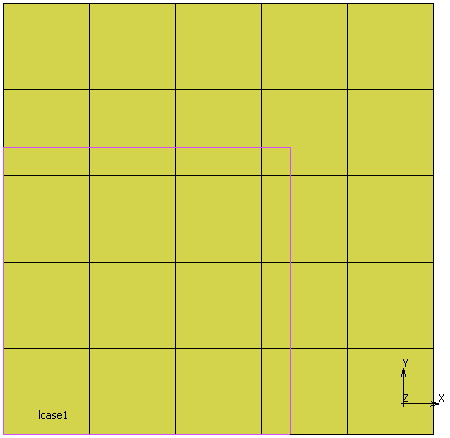
\includegraphics[width=0.5\textwidth]{C2Def.png}
	\caption{Resulting deformation of biaxial elongation}
	\label{fig:c2def}
\end{figure}

\subsection{Pure Shear}

Case 3 is a case of pure shear as defined by Kim \cite{Kim2015}. This case has no rigid body modes. This case has applications in causing angular extension or deformation. Four boundary conditions are applied. They are outlined in Table~\ref{tab:c3}.

% Please add the following required packages to your document preamble:
% \usepackage{booktabs}
\begin{table}[H]
\centering
\begin{tabular}{@{}lllc@{}}
\toprule
\multicolumn{1}{c}{\textbf{Label}} & \multicolumn{1}{c}{\textbf{Boundary}} & \multicolumn{1}{c}{\textbf{Constraint}} & \textbf{Direction} \\ \midrule
\textit{bc\_fd\_xy1} & Bottom edge & Fixed               & x \\
\textit{bc\_fd\_xy2} & Top edge    & Forced displacement & x \\
\textit{bc\_fd\_yx1} & Left edge   & Fixed               & y \\
\textit{bc\_fd\_yx2} & Right edge  & Fixed				 & y \\ \bottomrule
\end{tabular}
\caption{Pure shear boundary conditions \cite{Kim2015}}
\label{tab:c3}
\end{table}

The boundary conditions as applied in Marc Mentat to a template of 5x5 elements are illustrated in Figure~\ref{fig:c3bc}. The resulting deformation is illustrated in Figure~\ref{fig:c3def}. The original shape is outlined in pink.

\begin{figure}[H]
	\centering
	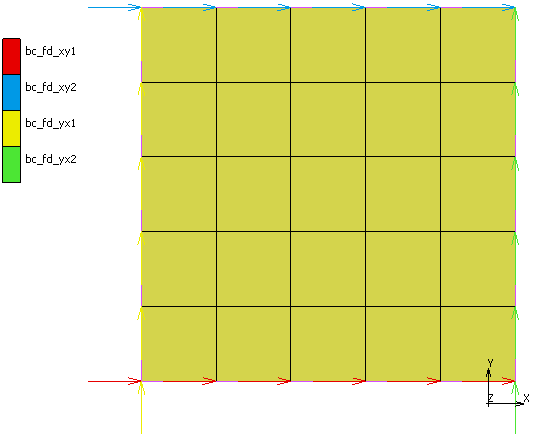
\includegraphics[width=0.5\textwidth]{C3BC.png}
	\caption{Pure shear boundary conditions as applied in Marc Mentat}
	\label{fig:c3bc}
\end{figure}

\begin{figure}[H]
	\centering
	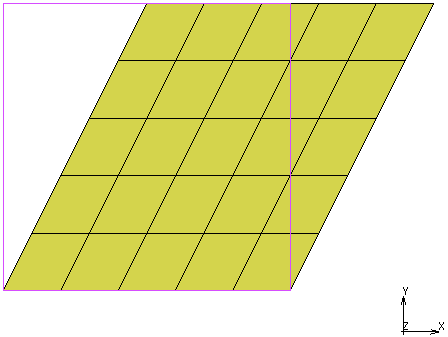
\includegraphics[width=0.5\textwidth]{C3Def.png}
	\caption{Resulting deformation of pure shear}
	\label{fig:c3def}
\end{figure}

\section{Material}

\subsection{Material Modeling}

The modeling of materials undergoing relatively large deformations is an active research field. Stored strain energy density may be used to compute stress in hyperelastic materials. The strain energy density is defined using invariants of strain. The three invariants are given as

\begin{equation}
	I_{1}=\lambda_{1}^{2}+\lambda_{2}^{2}+\lambda_{3}^{2}
\end{equation}

\begin{equation}
	I_{2}=\lambda_{1}^{2}\lambda_{2}^{2}+\lambda_{2}^{2}\lambda_{3}^{2}+\lambda_{3}^{2}\lambda_{1}^{2}
\end{equation}

and

\begin{equation}
	I_{3}=\lambda_{1}^{2}\lambda_{2}^{2}\lambda_{3}^{2}
\end{equation}

where $\lambda_{1}^{2}$, $\lambda_{2}^{2}$, and $\lambda_{3}^{2}$ are three eigenvalues. The undeformed state is used as the frame of reference. The three invariants will not change when using different coordinate systems. The three invariants must be positive for the deformation to be valid. The square root of $I_{3}$ measures the volume change of the material. $I_{3}=1$ if the material is incompressible \cite{Kim2015}.

The distortional strain energy density is defined as

\begin{equation}
	W_{1}\left ( I_{1},I_{2} \right )=\sum_{m+n=1}^{\infty}A_{mn}\left ( I_{1}-3 \right )^{m}\left ( I_{2}-3 \right )^{n}
\end{equation}

The Ogden model uses the principal stretches to define the distortional strain energy density as

\begin{equation}
	\label{eq:om}
	W_{1}\left ( \lambda_{1},  \lambda_{2}, \lambda_{3} \right )=\sum_{i=1}^{N}\frac{\mu_{i}}{\alpha_{i}}\left ( \lambda_{1}^{\alpha_{i}} + \lambda_{2}^{\alpha_{i}} + \lambda_{3}^{\alpha_{i}} \right )
\end{equation}

where $N$, $\mu_{i}$, and $\alpha_{i}$ are material parameters. $N$ is usually three. The principal stretches are the three eigenvalues of the deformation gradient. If the material is incompressible, the three principal stresses are not independent, meaning $\lambda_{1}\lambda_{2}\lambda_{3}=1$. The shear modulus is

\begin{equation}
	\mu=\frac{1}{2}\sum_{i=1}^{N}\alpha_{i}\mu_{i}
\end{equation}

The Ogden model correlates well with simple tension test data that is elongated up to 700\%. The model accommodates for slightly compressible behaviour and a nonconstant shear modulus \cite{Kim2015}.

\subsection{Material Selection}

Compliant and elastic materials are commonly used in the construction of soft robots. Three specific silicon-based rubbers that are readily accessible and affordable were characterized by Ellis \cite{Ellis2020}. These rubbers are outlined with basic material properties in Table~\ref{tab:ogdpar}.

% Please add the following required packages to your document preamble:
% \usepackage{booktabs}
% \usepackage{multirow}
\begin{table}[H]
\centering
\begin{tabular}{@{}crrr@{}}
\toprule
\multirow{2}{*}{\textbf{Parameter}} & \multicolumn{3}{c}{\textbf{Parameter Number}}                                                    \\ \cmidrule(l){2-4} 
                                    & \multicolumn{1}{c}{\textbf{1}} & \multicolumn{1}{c}{\textbf{2}} & \multicolumn{1}{c}{\textbf{3}} \\ \midrule
\multicolumn{4}{c}{\textbf{Ecoflex 00-30}}           \\ \midrule
$\mu$    & -0.0142909   & -3.64558e-06 & 9.59447e-08 \\
$\alpha$ & -5.22444     & -0.162804    & 11.3772     \\ \midrule
\multicolumn{4}{c}{\textbf{Mold Star 15 SLOW}}       \\ \midrule
$\mu$    & -6.50266e-06 & 0.216863     & 0.00137158  \\
$\alpha$ & -21.322      & 1.1797       & 4.88396     \\ \midrule
\multicolumn{4}{c}{\textbf{Smooth-Sil 950}}          \\ \midrule
$\mu$    & -0.30622     & 0.0283304    & 6.5963e-09  \\
$\alpha$ & -3.0594      & 4.59654      & 17.6852     \\ \bottomrule
\end{tabular}
\caption{Silicon-based Rubber Ogden Material Model Parameters \cite{Ellis2020}}
\label{tab:ogdpar}
\end{table}

Mold Star 15 SLOW is selected as the main material to be digitally modelled and manufactured for the purposes of the project. Mold Star 15's stiffness lies between EcoFlex and Smooth Sil's.  Mold Star 15 is selected because of its availability and properties. Mold Star 15 is deliverable to the premises where testing is to be done and available from a registered supplier. Additional properties are listed in Table~\ref{tab:gmp}.

\begin{table}[H]
	\centering
	\caption{Given Material Properties \cite{MoldStar}}
	\label{tab:gmp}
	\resizebox{\textwidth}{!}{%
		\begin{tabular}{@{}ccccc@{}}
		\toprule
		\textbf{Material} & \textbf{Cost/kg} & \textbf{Pot life (min)} & \textbf{Cure time (hr)} & \textbf{Tensile strength (MPa)} \\ \midrule
		Mold Star 15 SLOW & R332.00 & 50 & 4 & 2.7579 \\ \bottomrule
		\end{tabular}%
	}
\end{table}

Mold Star 15's long pot life allows for adequate time to prepare specimens thoroughly. The two components of the material need to be mixed according to a 1:1 ratio and stirred until completely mixed. The material then needs to be degassed, poured into the moulds, degassed again, and levelled.

Mold Star 15 has a hyper-elastic non-linear response. It is suitable for inflation while being capable of supporting itself at the relevant scale of construction.

The necessary properties to correctly digitally model Mold Star 15 are not available from the supplier. Testing is done according to ISO 37 and ISO 7743 standards for tensile and compression testing respectively to obtain data to construct an accurate Ogden model for the material \cite{ISO37,ISO7743}.

ISO 37 standards allow for the determination of the tensile stress-strain properties of vulcanised or thermoplastic rubbers. According to the given standards, dumb-bells of type 1A are cast and used used for testing purposes. Dumb-bell specimens are illustrated in Figure~.

\section{Testing Procedure}


